\def\year{2018}\relax
%File: formatting-instruction.tex
\documentclass[letterpaper]{article} %DO NOT CHANGE THIS
\usepackage{aaai}  %Required
\usepackage{times}  %Required
\usepackage{helvet}  %Required
\usepackage{courier}  %Required
\usepackage{url}  %Required
\usepackage{graphicx}  %Required
\usepackage{fullpage,enumitem,amsmath,amssymb,graphicx,listings, float,stmaryrd, textcomp}
\usepackage[noend]{algpseudocode}
\frenchspacing  %Required
\setlength{\pdfpagewidth}{8.5in}  %Required
\setlength{\pdfpageheight}{11in}  %Required
%PDF Info Is Required:
  \pdfinfo{
/Title (CS 257 Final Project)
/Author (Makai Mann)}
\setcounter{secnumdepth}{0}  
 \begin{document}
% The file aaai.sty is the style file for AAAI Press 
% proceedings, working notes, and technical reports.
%
\title{CS 257 Final Project \\ Towards Learning in SAT-based Bounded Model Checking}
\author{Makai Mann \\
21 March 2018
}
\maketitle
\begin{abstract}
SAT-based bounded model checking (BMC) is a state of the art formal verification approach for bug-finding. In a BMC run, a SAT solver is queried multiple times as the circuit is \textit{unrolled} over time. This sequence of queries is unsatisfiable until a potentially satisfiable call, when a counterexample is found. This paper explores machine learning techniques to learn from the unsat proofs of previous unrolls and applies the learned model to guide the SAT solver in subsequent unrolls. This project is focused on prototyping and thus makes use of existing, open source tools whenever possible.
\end{abstract}

\section{Introduction}
\noindent As digital circuits become increasingly complex, more and more of the time to produce a new design is spent in verification and validation. Formal approaches such as hardware model checking have arised as a popular complement to simulation based testing for catching bugs (and even proving correctness) earlier in the design process. Formal tools can reason over the design symbolically, which circumvents the primary challenge of simulation-based testing: the exponentially growing input space. Despite the relative success and broad adoption of these techniques in industry, formal tools still face scaling issues on larger designs. To prevent security flaws such as Meltdown and Spectre, and to save chip design companies huge sums of money spent on preventing and mitigating bugs, it is vital to address the scaling concerns of formal tools.

One of the most popular techniques is bounded model checking, which produces a bounded proof that a property holds. Typically, the bounded model checker iteratively increases the bound until it times out or finds a counter example trace. Intuitively, it seems that this sequence of calls to a formal solver might be related because each query is the same circuit unrolled over increasing time-steps. Therefore, it seems plausible that machine learning techniques could learn to guide the formal tool based on previous queries.

\section{Background}
This paper assumes basic knowledge of propositional logic. Below, I will begin by setting up the hardware model checking problem, describe the details of SAT-based bounded model checking, and finish by reviewing SAT solver's interpretation as resolution theorem provers. All of these topics are important for understanding the learning portion of this report.

\subsection{Hardware Model Checking}
Hardware model checking regards a digital circuit written in a representation language such as Verilog or VHDL as a symbolic finite state machine. Given the circuit description, some environmental assumptions and a property in a temporal logic, the model checking problems determines if the property holds. For the context of this report, I restrict focus to safety properties -- that a bad state is not reachable. It has been shown that other types of properties, such as liveness (something good eventually happens) can be reduced to safety checking \cite{biere}. Figure \ref{hwmc} shows the typical hardware model checking structure.

In the early days of model checking, explicit state techniques such as tableau methods were the focus. Since then, symbolic model checking has become the standard approach. Symbolic model checkers reason over sets of states as opposed to concrete states. SAT-based techniques encode the symbolic model checking problem into one or more SAT queries. This family of approaches includes algorithms which can definitely prove properties such as k-induction and property directed reachability, as well as bounded techniques such as bounded model checking, which can only find bugs. For many classes of circuits, bounded model checking is the fastest approach for finding obscure bugs.

\begin{figure}[H]
\begin{center}
  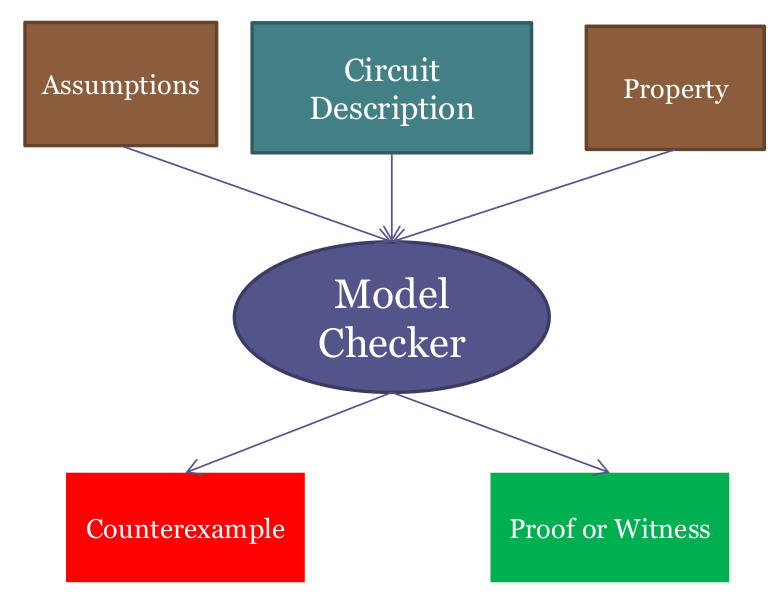
\includegraphics[scale=0.2]{hwmc.png}
  \caption{Hardware Model Checking setup}
  \label{hwmc}
\end{center}
\end{figure}

\subsection{SAT-based Bounded Model Checking}
In SAT-based bounded model checking, each bit of the circuit is given a SAT literal and the combinational logic is represented with SAT formulas. To capture the behaviour of sequential elements, the literals are duplicated for each clock cycle and constrained with a transition relation that models the circuit behaviour.

Formally, $M := <V, I, T>_k$ describes the SAT encoding at bound $k$. Where, 
\begin{equation*}
\begin{split}
V &= \{B_0^{(0)} \dots B_{n}^{(0)} \dots B_{n}^{(k)}\} \text{, the SAT variables} \\
I &= \text{The formula describing the initial state} \\
T &= \text{The formula capturing the relation} \\
&  \ \  \ \  \ \  \text{between current and next state elements}
\end{split}
\end{equation*}

Then by checking if $M \models P$ for some property formula $P$, we are checking if there is any trace violating the property in $k$ time-steps.

\subsubsection{2-bit Counter Example}

A simple 2-bit counter with the clock abstracted (next states are the state after a full clock cycle) can be described at $k=1$ as follows:

\begin{equation*}
\begin{split}
V &= \{C_1^0, C_0^0, C_1^1, C_0^1\} \\
I &= \neg C_0^1 \wedge \neg C_0^0 \\
T &= C_0^1 \oplus C_0^0 \wedge \\
& \neg (C_1^1 \oplus (C_1^0 \oplus C_0^0))
\end{split}
\end{equation*}
This starts the counter at $00$ in the initial state and the transition relation evaluates to true exactly when the next state is the current state incremented by one. As $k$ increases, the transition relation is repeated for each pair of related states. This large propositional formula is then converted to conjunctive normal form (CNF) and passed to a SAT solver along with the negated property. A \textit{clause} refers to a disjunction of literals in CNF. A satisfiable result gives a model assignment which is a counter example trace. An unsatisfiable result means the property holds up until bound $k$.  

Thus, in a typical bounded model checking run, there is a sequence of $k-1$ unsatisfiable queries to the SAT solver, after which there is either a timeout or one satisfiable query, in which case a bug is identified and the SAT model gives a counterexample trace. Thus, to speed up bounded model checking it behooves us to focus on unsatisfiable queries, because they make up the bulk of the effort. Furthermore, unsatisfiable queries are able to produce a lot of potentially useful data in the form of an unsat proof.

\subsection{SAT Solvers as Resolution Theorem Provers}

A common form for a proof of unsatisfiability is a resolution refutation proof. This proof is represented as a DAG where each node is a clause. Each node is either a leaf, meaning it was part of the original clauses given in the SAT query, or has two parents. The parents are each clauses that have been resolved on a literal to produce the child clause. A resolution DAG always ends in the empty clause which demonstrates that the original queries were unsatisfiable. While resolution is a sound and complete technique for proving unsatisfiability, there are exponentially many ways of producing clause resolutions and in practice this approach does not perform well. Rather, the most common modern approach is to use a conflict-driven clause learning (CDCL) SAT solver.

Although CDCL SAT solvers do not employ clause resolution very often, they can still produce resolution refutation proofs. In fact, it has been shown that CDCL solvers p-simulate general resolution for propositional logic \cite{cdclres}.

In the process of solving a SAT problem, CDCL solvers find \textit{conflicts}: a known clause from the database which is falsified by the current assignment of literals. Once a conflict has been found, it can be modified by resolving on literals forced by unit propagation in the current assignment trail. This produces a learned clause which is then added to the database, preventing the SAT solver from exploring this part of the space again. For more detailed coverage of this topic, see \cite{satres}.

\subsubsection{Antecedent Graphs}

Resolution proofs can grow exponentially large, thus the SAT community developed a trace format which represents a resolution proof in a more compact format. The trace format represents the proof as an antecedent graph where there are edges between clauses and the learned clauses they produce. Unlike a resolution proof, each node in the graph can have more than two parents. The parents are not required to be in any particular order, but by applying clause resolution between the parents, it is possible to derive the child.

The learning phase of this project will take a resolution proof or antecedent graph as inputs and attempt to learn some underlying structure of the circuit.

\subsection{Supervised Learning}
Supervised learning aims to construct a classification or regression function based on a set of data points and their associated labels. The reader is assumed to be familiar with basic supervised learning techniques. Thus, the learning algorithms are omitted from the background section. The curious reader can refer to \cite{Murphy} for a complete introduction.

\section{Learning from Previous Queries}

Given an unsat proof from the $(k-1)th$ bounded model checking call, a machine learning algorithm can learn a scoring function which can identify useful clauses at bound $k$. Then, a procedure will generate many resolvents and the scoring function can be used to decide which resolvents to keep. Furthermore, the function can actually be used to direct the clause resolution online towards more useful resolvents.

The discussion below starts with a description of the normal form transformation used for all SAT literals, continues with various feature selection techniques and concludes with the method for assigning labels. The majority of this project consisted of defining and producing the right data, and only then trying multiple algorithms for model learning.

\subsection{Normal Form}
The goal is to learn to score useful clauses, thus the input to the scoring function will be a clause in some processed form. The first fundamental transformation I applied was mapping all literals in a clause to an equivalence class.

In the BMC query, there is a new literal for every bit in the circuit for every time step. Thus, rather than including all literals, I chose a representative for each physical wire and mapped all literals to that one literal. For example, the following expressions (given in SMT-LIB notation) would each receive a literal in the SAT transformation, and would be mapped to a normal form:

\begin{equation*}
\begin{split}
&\text{(= wrPtr@4 (+ wrPtr@3 \#b0001))} \\
&\to \text{(= wrPtr@(k+1) (+ wrPtr@k \#b0001))} \\
&\text{(= wrPtr@3 (+ wrPtr@2 \#b0001))}\\
&\to \text{(= wrPtr@(k+1) (+ wrPtr@k \#b0001))}
\end{split}
\end{equation*}

\noindent where "@" is a naming scheme which annotates the signal name with the time-step.

In practice, the representative literal is chosen arbitrarily as the first instance of a signal. 

The normal form is important so that the machine learning algorithm does not have to recover temporal relations between these literals that is already known. This transformation is inspired by other symbolic model checking techniques such as Binary Decision Diagram techniques and Property Directed Reachability (PDR). Both of these approaches are based on fixpoint computations which iteratively calculate all reachable states over the transition relation without unrolling the circuit. Instead they only look at the current and next state abstractly. PDR in particular is similar to this normal form transformation in that it extends the trace length, but adds each new reachable state to the abstract representation.

The normal form of a clause is simply the clause produced by mapping all of its literals to their normal form, and sorting them in ascending order. Sorting the literals in the clause ensures that a given clause has only one representation.

\subsection{Features}

\subsubsection{Sampled Literals}
\subsubsection{One-Hot Literals}
\subsection{Labels}
\subsubsection{Unsat Trace}
\subsubsection{Resolution Proof}
\subsubsection{Classification vs. Regression}
\section{Implementation}
\subsection{Toolflow}
\subsection{Data Collection}
\subsection{Learning Framework}
\subsubsection{Machine Learning Algorithms}
\subsection{Case Study Benchmark}
\section{Results}
\section{Analysis}
\section{Related Work}
\section{Conclustion}
\section{Acknowledgements}

\bibliographystyle{aaai}
\bibliography{report}

\end{document}